\chapter{Interferência entre Máquinas Virtuais}\label{chap:interferencia}

\section*{}


% Este capítulo deve começar por fazer uma apresentação detalhada do
% problema a resolver\footnote{Na introdução a apresentação do
%   problema foi breve.} podendo mesmo, caso se justifique,
% constituir-se um capítulo com essa finalidade.

% Deve depois dedicar-se à apresentação da solução sem detalhes de
% implementação. 
% Dependendo do trabalho, pode ser uma descrição mais teórica, mais
% ``arquitetural'', etc.

Os sistemas de virtualização são a principal tecnologia para o funcionamento das nuvens computacionais. Os hipervisores controlam a alocação de recursos a cada máquina virtual, no entanto existem recursos fisicamente partilhados, impossíveis de distribuir uniformemente, sendo a sua utilização ditada pelos controladores de \textit{hardware}. Não sendo possível aos hipervisores resolver esta alocação, cada VM alocada pode-se apoderar da totalidade dos recursos partilhados e impedir as restantes de executarem o seu trabalho. O trabalho desta dissertação pretende minimizar estas ocorrências, através do estudo das interferências e executar uma alocação de tarefas a cada nó consciente do impacto das mesmas no rendimento das tarefas que já se encontram em execução ou em espera nesse nó.

\section{Dados de Interferência}

Na Figura \ref{fig:modeloshell} é possível visualizar o rendimento de execução de dois comandos de \textit{shell} em máquinas virtuais separadas\footnote{As máquinas virtuais possuem recursos iguais e o hospedeiro possui capacidade igual ou superior à soma das duas.}. O resultado é normalizado ao tempo de execução do comando \textbf{grep} e os restantes valores são obtidos através das fórmulas . O desempenho da tarefa \textbf{grep} em conjunto com a \textbf{povray} tem um rendimento perto de perfeito, quase atingindo o valor 2. No entanto todas as outras combinações degradam o desempenho, atingindo um mínimo quando dois \textbf{grep} são executados paralelamente. 

\begin{figure}[t]
  \begin{center}
    \leavevmode
    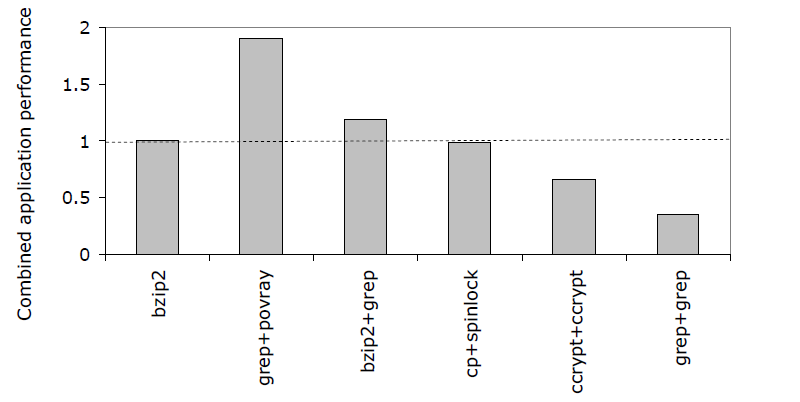
\includegraphics[width=0.86\textwidth]{interferenciashell.png}
    \caption{Tempo de execução normalizado de duas máquinas virtuais a executar commandos da \textit{shell}. Fonte: \cite{koh2007analysis}}
    \label{fig:modeloshell}
  \end{center}
\end{figure}

\section{Abordagem}



% Neste capítulo apresentam-se exemplos de formatação de figuras e
% tabelas, equações e referências cruzadas.

% Apresenta-se de seguida um exemplo de equação, completamente fora do contexto:
% \begin{eqnarray}
% CIF_1: \hspace*{5mm}F_0^j(a) &=& \frac{1}{2\pi \iota} \oint_{\gamma} \frac{F_0^j(z)}{z - a} dz\\
% CIF_2: \hspace*{5mm}F_1^j(a) &=& \frac{1}{2\pi \iota} \oint_{\gamma} \frac{F_0^j(x)}{x - a} dx \label{eq:cif}
% \end{eqnarray}

% Na Equação~\ref{eq:cif} lorem ipsum dolor 

% A arquitetura do visualizador assenta sobre os seguintes conceitos
% base~\cite{kn:ZPMD97}: 

% \begin{itemize}
% \item \textbf{Componentes} --- Suspendisse auctor mattis augue \emph{push};
% \item \textbf{Praesent} --- Sit amet sem maecenas eleifend facilisis leo;
% \item \textbf{Pellentesque} --- Habitant morbi tristique senectus et netus.
% \end{itemize}


% É apresentado na Figura~\ref{fig:arch} %da página~\pageref{fig:arch}
% um exemplo de figura flutuante.

% \begin{figure}[t]
%   \begin{center}
%     \leavevmode
%     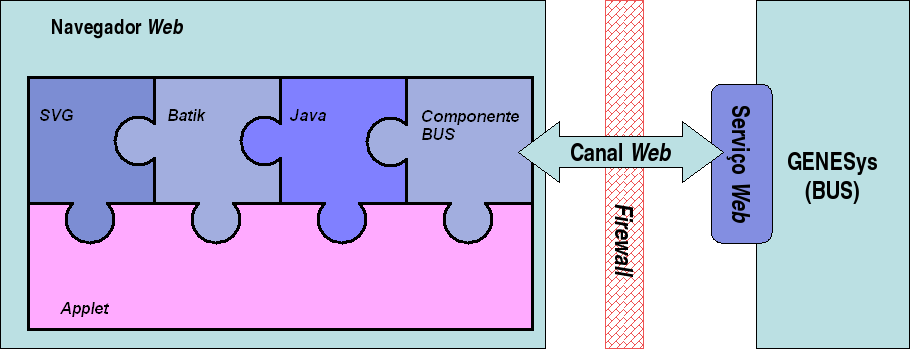
\includegraphics[width=0.86\textwidth]{puzzle}
%     \caption{Arquitectura da Solução Proposta}
%     \label{fig:arch}
%   \end{center}
% \end{figure}


% É apresentado na Tabela~\ref{tab:exemplo1} um exemplo de tabela
% flutuante e na Tabela~\ref{tab:exemplo2} um exemplo de tabela
% flutuante, um pouco mais complicada.

% \begin{table}[t]
%   \centering
%   \caption{Uma Tabela Simples}
% \begin{tabular}{| l | p{45mm} |}
% 	\hline
% \textbf{Acrónimo} & \textbf{Significado}\\
% 	\hline
% 	\hline
%         ADT   & \emph{Abstract Data Type}\\\hline
%         ANDF  & \emph{Architecture-Neutral Distribution Format}\\\hline
%         API   & \emph{Application Programming Interface}\\
% 	\hline
% \end{tabular}
%   \label{tab:exemplo1}
% \end{table}



% \begin{table}[t]
%   \centering
%   \caption{Uma Tabela Mais Complicada}
% \begin{tabular}{|c|r@{.}lr@{.}lr@{.}l||r|}
% 	\hline
% \multicolumn{8}{|c|}
% 	{\rule[-3mm]{0mm}{8mm}Iteração $k$ de $f(x_n)$} \\
% \textbf{\em k}
% 	& \multicolumn{2}{c}{$x_1^k$}
% 	& \multicolumn{2}{c}{$x_2^k$}
% 	& \multicolumn{2}{c||}{$x_3^k$}
% 	& comentários \\ \hline \hline
% 0   & -0&3                 & 0&6                 &  0&7   & - \\
% 1   &  0&47102965 & 0&04883157 & -0&53345964  & $\delta<\epsilon$ \\
% 2   &  0&49988691 & 0&00228830 & -0&52246185  & $\delta < \varepsilon$ \\
% 3   &  0&49999976 & 0&00005380 & -0&523656   &   $N$ \\
% 4   &  0&5                 & 0&00000307 & -0&52359743  & \\
% \vdots	& \multicolumn{2}{c}{\vdots}
% 	& \multicolumn{2}{c}{$\ddots$}
% 	& \multicolumn{2}{c||}{\vdots}  & \\
% 7   &  0&5   & 0&0    & \textbf{-0}&\textbf{52359878}
% 		 & $\delta<10^{-8}$ \\ \hline
% \end{tabular}
%   \label{tab:exemplo2}
% \end{table}



\section{Resumo e Conclusões}


